\documentclass{beamer}
\usetheme{Boadilla}
\usepackage{essay-def}
\usepackage{bm}
\usepackage{amsfonts}
\usepackage{amssymb}
\usepackage{amsmath}
\usepackage{amsthm}
\usepackage{comment}
\usepackage{subcaption}
\usepackage{geometry}
\newcommand{\JX}[1]{{\color{red}{$^{\text{JX}}$[#1]}}}
\geometry{left=1cm,right=1cm}
    \title[Distribution Shift]{Distribution shift in machine-learning augmented fluid simulation}
\author[DS grp]{Distribution shift review group}
\date{18th Sep, 2023}
\begin{document}
\par \setlength{\parindent}{2em}

\begin{frame}
\titlepage

\end{frame}

\begin{frame}
	\textbf{Content:}
	\begin{itemize}
		\item * Brief overview of machine-learning augmented fluid simulation
		\item * Data generation and preprocessing
		\item * Network model and simulation framework design
		\item * Loss function and training algorithm
		\item * Performance evaluation
	\end{itemize}
\end{frame}

\begin{frame}{Simulation framework}
	To be concrete and simple, suppose the task is given as
	\begin{equation}
		X_{t+\Delta t} = X_t + NN(X_t; \theta),
	\end{equation}
	where $NN(X_t; \theta)$ is usually learned under supervision. The ``rollout'' trajectory produced by iteratively applying learned model for $K$ steps is denoted $(\wht X_0, \wht X_1, \cdots, \wht X_n)$, where $\wht X_0 = X_0$ represents initial conditions given as input.
	\begin{figure}[ht]
		\centering
		\centerline{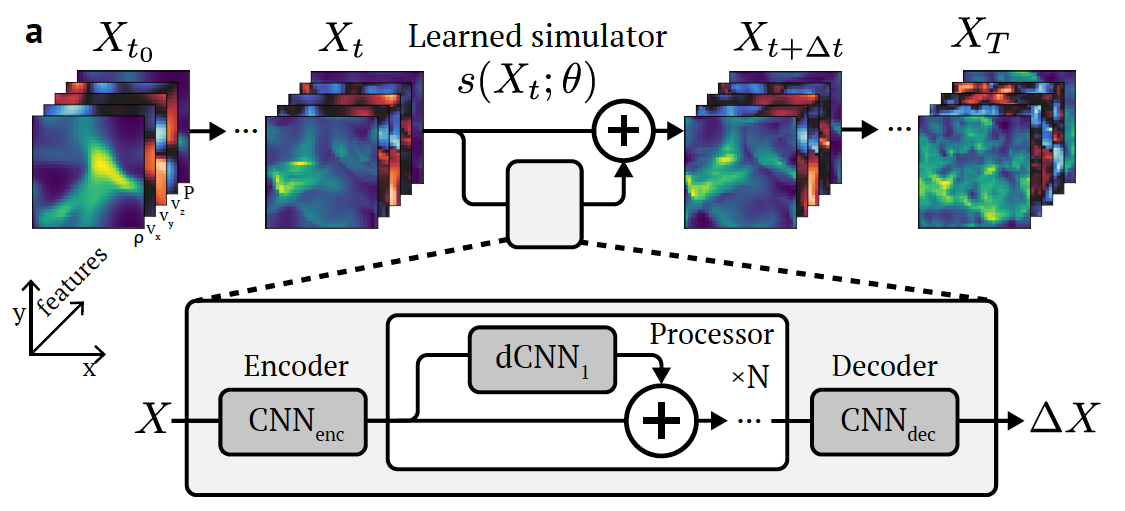
\includegraphics[width=.8\linewidth]{fig/framework.png}}
		\caption{Framework}
	\end{figure}
\end{frame}

\begin{frame}{Difficulties in the fluid simulation}
	There are several outstanding difficulties in the fluid simulation:
	\begin{itemize}
		\item * Intrinsic nature of chaotic dynamics: KS equation, isotropic turbulence, etc.
		\item * High resolution grid results in extremely high dimension dynamics
		\item * There does not exist a unified performance criterion.
	\end{itemize}
	\JX{\small After stating each of the difficulties, trying to answer whether any of them can be 
	addressed with the help of machine learning, especially when you are talking about your own work}
\end{frame}

\begin{frame}{Difficulties in the fluid simulation}
	\begin{figure}[ht]
		\centering
		\centerline{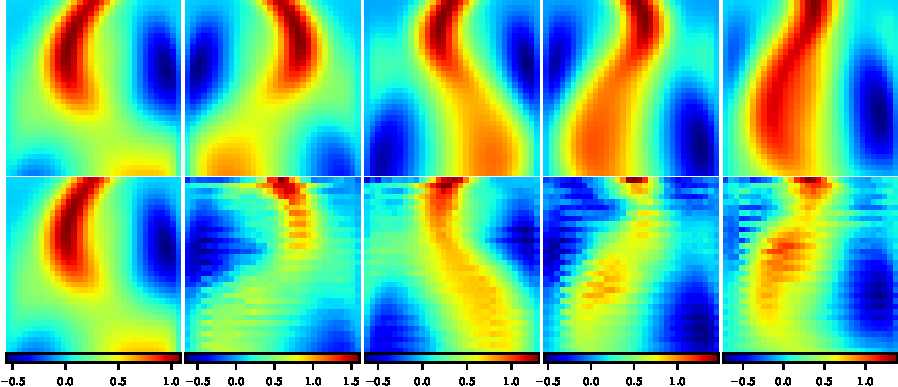
\includegraphics[width=\linewidth]{fig/ds1.pdf}}
		\centerline{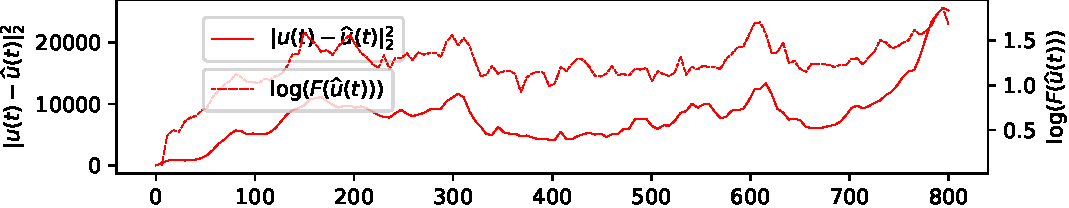
\includegraphics[width=\linewidth]{fig/ds2.pdf}}
		\caption{Difficulty of fluid simulation}
	\end{figure}
\end{frame}

\begin{frame}{Data generation}
	Current methodology, use a high-fidelity numerical solver to generate, 
	including random initialized state, warmup, trajectory, labeling.

	There are many ``hyperparameters'' that can be tuned to generate a SciML dataset:
	\begin{itemize}
		\item Initialization: sampled from some distribution.
		\item Sampling: same as the time discretization of the numerical solver
		\item Warmup time: truncated the first several iterations
	\end{itemize}
	\JX{\small Warmup and sampling are more or less related, e.g. considering the 
	simulating of a dynamics with an invariant distribution. In Lin Bo's work where
	they try to learn the transition at the transition between two metastable states
	which corresponds to rare events, we indeed hope the data to be distributed uniformly 
	instead of concentrating in certain area.}
\end{frame}

\begin{frame}{Data generation}
	\begin{figure}[ht]
		\centering
		\centerline{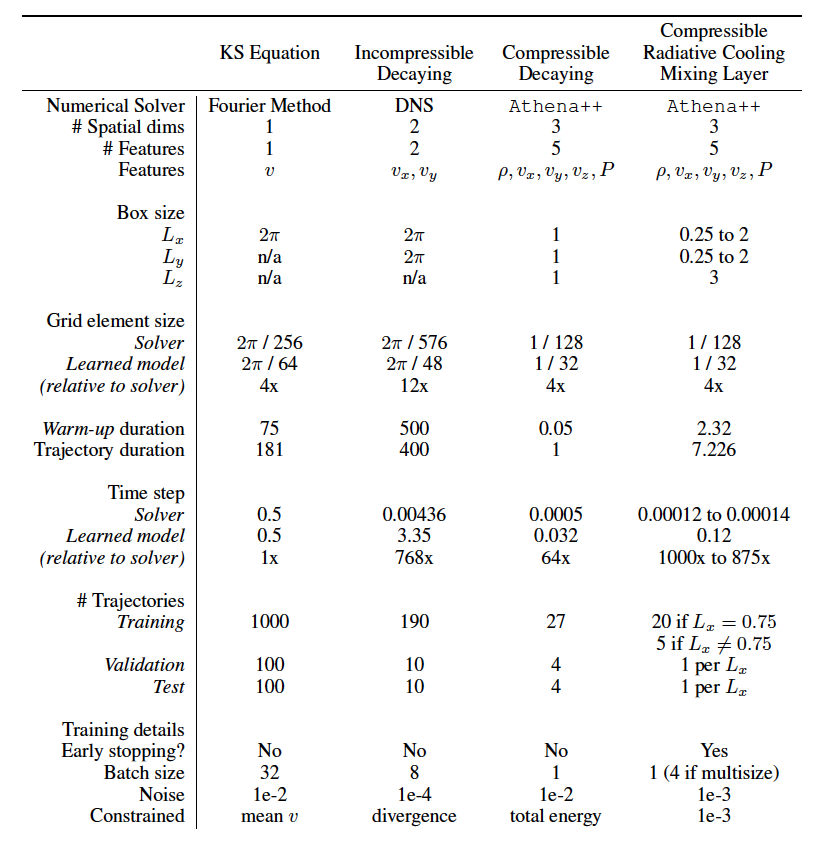
\includegraphics[width=.6\linewidth]{fig/dataset.png}}
		\caption{Dataset details.}
	\end{figure}
\end{frame}

\begin{frame}{Data preprocessing}
	There are several methods, here we list three
	\begin{itemize}
		\item * No preprocessing: physical information is important.
		\item * Same as most statistical learning, entrywise preprocessing: 
		resolve the issue of multiscale in different components.
		\item * Similar to some CV task: group all the entries together. 
	\end{itemize}
	\begin{figure}[ht]
		\centering
		\centerline{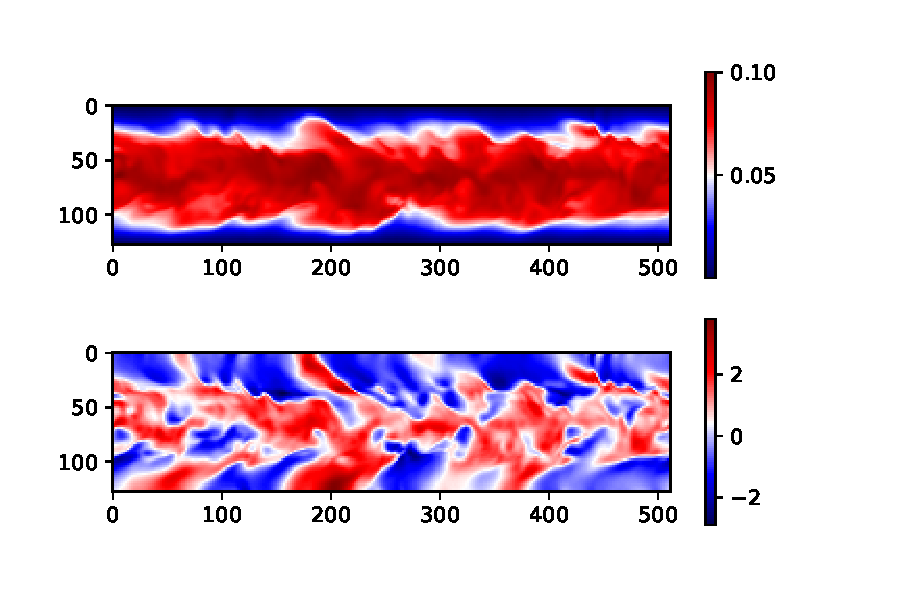
\includegraphics[width=.6\linewidth]{fig/data-std.pdf}}
		\caption{Comparison of data preprocessing: No preprocessing v.s. entrywise preprocessing}
	\end{figure}
\end{frame}

\begin{frame}{Data preprocessing}
\begin{figure}[ht]
	\centering
	\begin{subfigure}{0.5\linewidth} % Adjust the width as needed
		\centering
		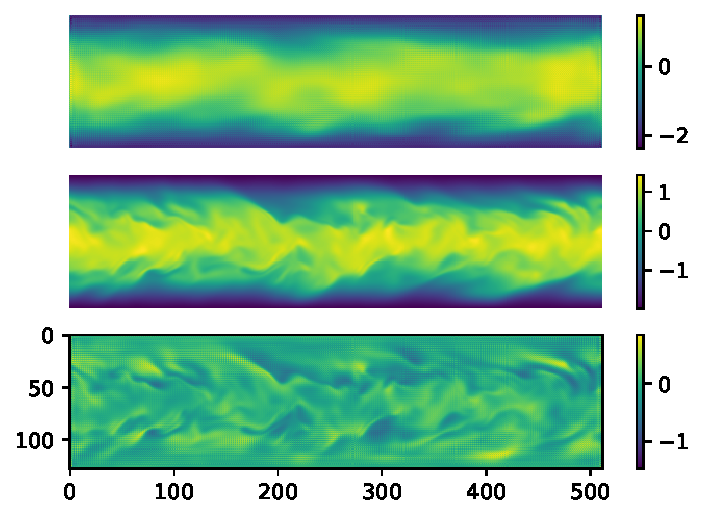
\includegraphics[width=\linewidth]{fig/ED-std.pdf}
		\caption{Data with preprocessing}
	  \end{subfigure}%
	  \begin{subfigure}{0.5\linewidth} % Adjust the width as needed
		\centering
		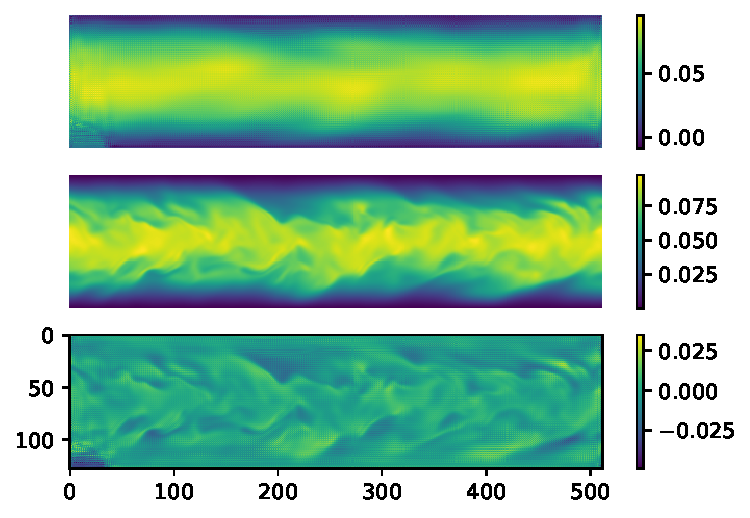
\includegraphics[width=\linewidth]{fig/ED.pdf}
		\caption{Data without preprocessing}
	  \end{subfigure}
	  \caption{Comparison of data preprocessing}
\end{figure}
\end{frame}

\begin{frame}{Data Preprocessing}
	Which of the following data form is most similar to dynamical fluid prediction?
	\begin{itemize}
		\item * Image 
		\item * Video
		\item * Sequence
	\end{itemize}

	\textbf{Preprocessing should respect physical properties.}

	\textbf{The effect of data generation and preprocessing on simulation results and distribution shift is seldomly studied.}
\end{frame}

\begin{frame}{Network architecture}
	The backbone for most network models is UNet
	\begin{figure}[ht]
          \centering
          \centerline{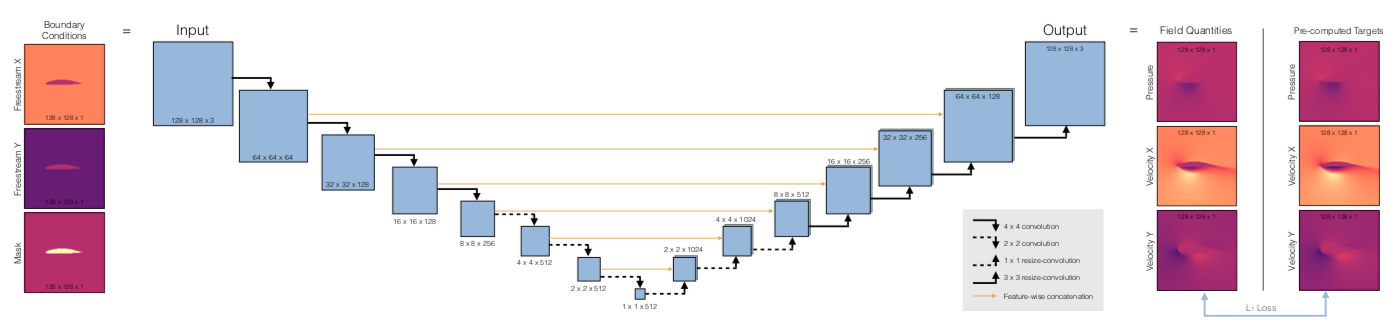
\includegraphics[width=1.1\linewidth]{fig/Unet.png}}
          \caption{U-net structure for flow prediction\footnotemark}
\end{figure}

	It is similar to the autoencoder, performing non-linear dimension reduction.
	At the same time it could account for interaction at different scale.

	There is large literature using GCN for irregular grid.
	\footnotetext{Thuerey, Nils, et al. "Deep learning methods for Reynolds-averaged Navier–Stokes simulations of airfoil flows." AIAA Journal 58.1 (2020): 25-36.}
\end{frame}

\begin{frame}{Network architecture: TF-Net}
	The turbulent flow net\footnotemark  learns the temporal and spatial
	filter which follows the methodology of RANS-LES hybrid simulation.
	\begin{figure}[ht]
		\centering
		\centerline{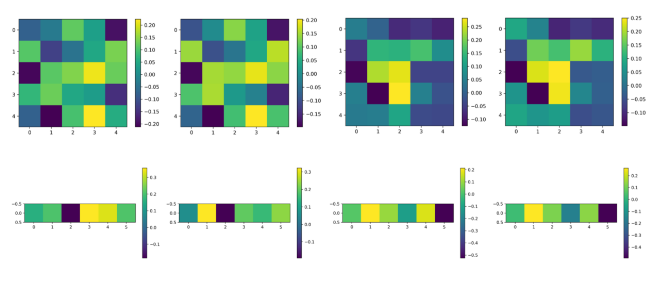
\includegraphics[width=1\linewidth]{fig/filterlearned.png}}
		\caption{Learned spatial and temporal filter\footnotemark}
\end{figure}
	
	\footnotetext{Wang, Rui, et al. "Towards physics-informed deep learning for turbulent flow prediction." Proceedings of the 26th ACM SIGKDD International Conference on Knowledge Discovery \& Data Mining. 2020.}
\end{frame}

\begin{frame}{Simulation framework}
	Two mainstreams:
	\begin{itemize}
		\item Viewing fluid prediction as an image task, using large
		CNN as parametrized model\footnotemark.
		\item Using neural network to determine parameters for empirical model\footnotemark, more similar to the inverse problem and turbulence modeling.
	\end{itemize}
	\footnotetext{Stachenfeld, Kimberly, et al. "Learned coarse models for efficient turbulence simulation." arXiv preprint arXiv:2112.15275 (2021).}
	\footnotetext{Wang, Rui, et al. "Towards physics-informed deep learning for turbulent flow prediction." Proceedings of the 26th ACM SIGKDD International Conference on Knowledge Discovery \& Data Mining. 2020.}
\end{frame}

\begin{frame}{Loss function}
	The basic choice is to train with one-step supervision under MSELoss.
	\begin{equation}
		l(\theta) = \mbE_{X\sim \rho}\norml NN(X_t;\theta) - \Delta X_t \normr_2^2
	\end{equation}
	Physics-informed constraints are used as regularization, such the divergence-free properties of the incompressible fluid simulations,
	\begin{equation}
		l(\theta) = \mbE_{X\sim \rho}\norml NN(X_t;\theta) - \Delta X_t \normr_2^2 + \norml \nabla \cdot X_{t+\Delta t} \normr_2^2
	\end{equation}

	In fluid mechanics community, sometimes the accuracy of fluid statistics such as energy spectrum is more important than the trajectorywise accuracy.
	If this becomes the ultimate goal, is there a notion of distribution shift?
\end{frame}

\begin{frame}{Stability via adding noise}
	Stability issue: small errors can accumulate over rollouts and lead to a domain shift.

	Add Gaussian noise to the input to robustify the learned models,
	which is similar to the adverserial training in CS literature. 
	And the size of the noise serve a role in bias-variance trade-off.
	\begin{equation}
		\begin{aligned}
			X_t + \epsilon & \rightarrow \Delta X_t, 		\\
			X_t + \epsilon & \rightarrow \Delta X_t + \epsilon.
		\end{aligned}
	\end{equation}
	This is presumably because the training distribution has broader support and the model is optimized to map deviant inputs back to the training distribution.
	\JX{\small Adding noise during the training makes more sense, otherwise there is 
	no difference bewteen adding noise in simulating the trajectory, or simply including
	observation noise in collecting the trajectory data.}
\end{frame}

\begin{frame}{Stability via adding noise}
	\begin{figure}[ht]
		\centering
		\centerline{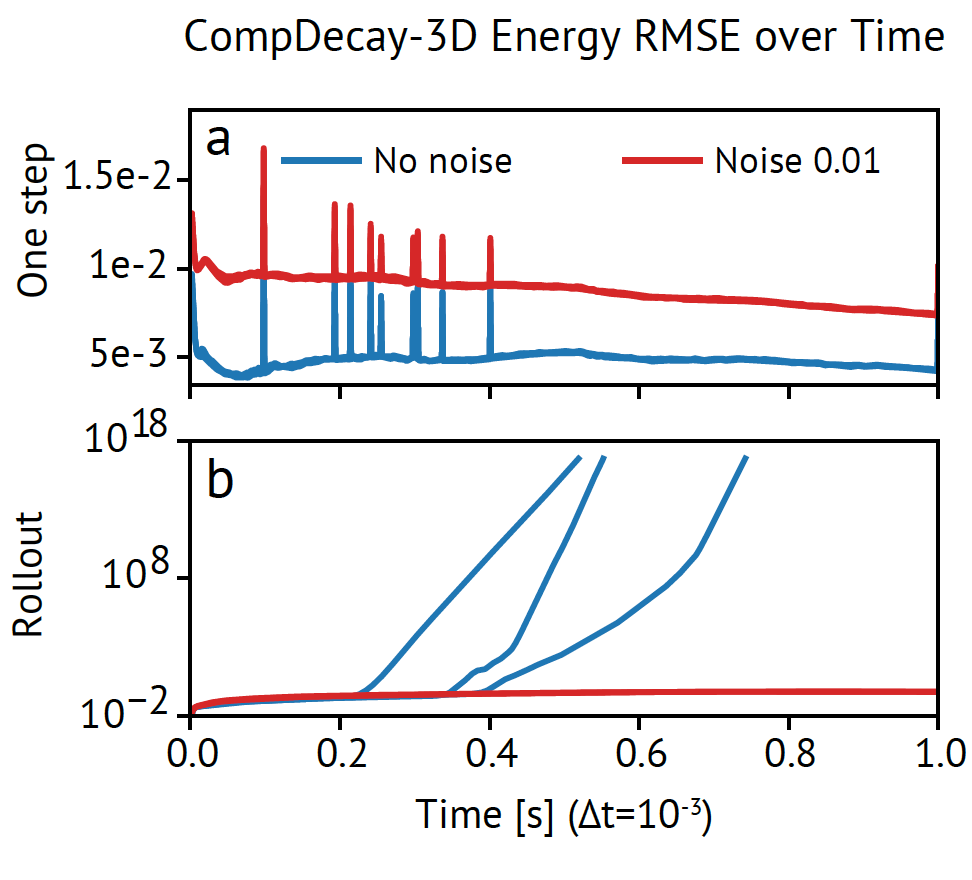
\includegraphics[width=.6\linewidth]{fig/adverserial.png}}
		\caption{Effect of training with artificial noise\footnotemark}
\end{figure}
\footnotetext{Stachenfeld, Kimberly, et al. "Learned coarse models for efficient turbulence simulation." arXiv preprint arXiv:2112.15275 (2021).}
\end{frame}

\begin{frame}{Stability via Temporal coarsening}
	An advantage of learned simulators is that they can exploit a much larger step size than the 
	numerical solver, as they can discover efficient updates that capture relevant dynamics on larger 
	timescale. This allows for faster simulation.

	Choosing the timestep also has a trade-off: while larger
	time step has greater error each step, smaller step size 
	has more iteration leading to unstability.
	\JX{Think about if there is any similar phenomena in classical
	numerical analysis, Prof. Li suggests thinking about the 
	conditional stability of the classical numerical schemes, e.g.
	FTCS is unconditionally unstable for transport equation, upwind 
	scheme is conditionally stable, and many other similar criterion 
	for numerical scheme of parabolic equation}
\end{frame}

\begin{frame}{Stability via Temporal coarsening}
	\begin{figure}[ht]
		\centering
		\centerline{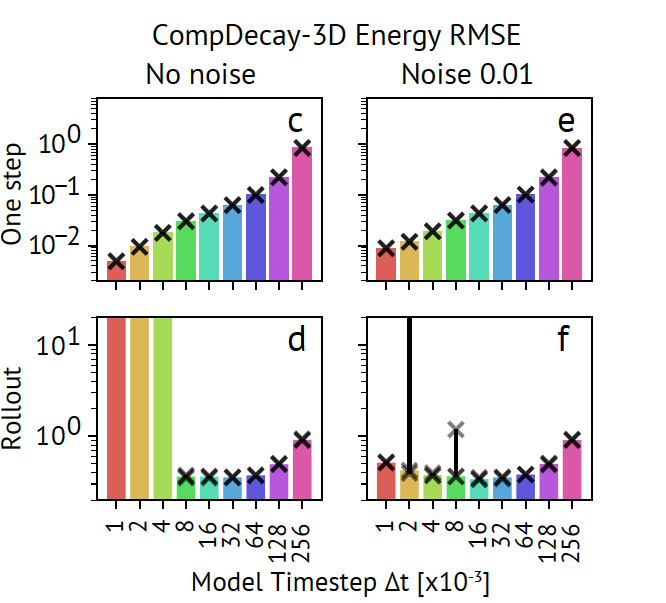
\includegraphics[width=.6\linewidth]{fig/Tcoarsening.png}}
		\caption{Effect of temporal coarsening\footnotemark}
\end{figure}
\footnotetext{Stachenfeld, Kimberly, et al. "Learned coarse models for efficient turbulence simulation." arXiv preprint arXiv:2112.15275 (2021).}
\end{frame}

\begin{frame}{Performance evaluate}
	\begin{itemize}
		\item Accuracy is not the only thing we care about in fluid simulation. 
		Sometimes they do not even care about accuracy as the dynamics is chaotic.
		\begin{equation}
			\int_{[0, T]}\norml \wht X_t - X_t \normr_2^2dt
		\end{equation}
		\item Statistics \& physical quantities: turbulent kinetic energy, energy spectrum
		\begin{equation}
			\begin{aligned}
				\text{TKE:}\quad \frac{\sum_0^T \lb (u_t - \bar{u})^2 + (v_t - \bar{v})^2 \rb}{2T}.
			\end{aligned}
		\end{equation}
		\textbf{If we only care these physical quantities, is distribution shift still 
		an issue here? If it is, how should we identify or quantify it?}
	\end{itemize}
	\JX{\tiny Here, distribution shift becomes something which is too special or narrow. 
	The more general terminology we should use should be something like mismatch, 
	which coule either represents the mismatch of the training and testing distribution 
	or between the train loss function and the loss test function, e.g. train with $L^2$ 
	while in inference we only cares about the behavior at the extreme value pts.}
\end{frame}

\end{document}